\documentclass[11pt,letter]{article}
\usepackage[top=1.00in, bottom=1.0in, left=1.1in, right=1.1in]{geometry}
\usepackage{graphicx}
\usepackage{natbib}
\usepackage{amsmath}

\def\labelitemi{--}
\parindent=10pt

\begin{document}
%\bibliographystyle{/Users/Lizzie/Documents/EndnoteRelated/Bibtex/styles/besjournals}
\bibliographystyle{/Users/aileneettinger/citations/Bibtex/styles/amnat.bst}

\renewcommand{\refname}{\CHead{}}


{\bf Titles}

Chilling dominates tree budburst in controlled climate experiments, but not in the great outdoors
Chilling outweighs photoperiod and forcing cues in temperate trees in experiments, but not in natural systems


\begin{abstract}
Decades of research on woody species highlight how three major cues shape spring phenological events (e.g., budburst and leafout): forcing (warm temperatures, generally occurring in the late winter and early spring), daylength (photoperiod) and chilling (cool temperatures, generally occurring in the fall and late winter). How pervasive these cues are and whether some species are effectively governed by only one or two cues is a critical area of climate change biology research, as it would shape how complex responses to warming will be. Here we use a global meta-analysis of all published growth chamber studies to test for the relative effects of these three major cues across XX species. We find they almost all show these cues, making climate change responses complex. 
\end{abstract}

\section* {Text so far...}

% From Lizzie: I set the \parindent to 10pt in preamble since you use it (I usually just end paragraphs with \\ versus than start them with \par). 
\par For decades, plant phenology has been one of the most reported and consistent biological imprints of climate change \citep{IPCC:2014sm}, with many temperate plants leafing and flowering earlier with rising temperatures (cites). Understanding such shifts is important as phenology shapes a suite of ecosystem services, including pollination and carbon sequestration, and scales up to impact projections of climate change itself. 

\par As research interest in phenology has progressed, critical discrepancies and uncertainties in our understanding have emerged. Though responses to warming are consistent on average \citep{Wolkovich:2012n}, they show high variation across species and sites (cites). Furthermore, long-term observational studies provide increasing evidence that sensitivities of phenology to temperature are weakening in recent decades \citep{yu2010}. In Europe, recent work from some of the most well-studied tree species shows declining responses to temperature, suggesting that the long-term trend towards ever-earlier springs may be stalling \citep{fu2015}. The authors, and others, suggest that responses to other environmental cues underlie these declining temperature sensitivities.

\par Fundamental research in phenology outlines three major cues known to shape spring phenology \citep{chuineJTB}: chilling (cool temperatures, generally occurring in the fall and late winter), forcing (warm temperatures, generally occurring in the late winter and early spring), and daylength (photoperiod). Research suggests these cues drive spring phenology for many temperate woody species (CITES), but there is strong debate over how prevalent these cues are across species (KornerBasler etc.) and which cues dominate (CITES). Given the declining response to temperature observed in long-term observational studies \citep{fu2015}, a number of papers have tried to tease out evidence of unfufilled chilling or daylength cues in recent years (CITES), but such work must overcome the fundamental challenge that all three major cues are often strongly correlated in nature. During the transition from winter to spring at many temperate latitudes, air temperatures increase (i.e., forcing increases) at the same time that daylength is increasing; likewise, winters with low amounts of chilling are often correlated with warmer springs, and thus higher forcing.  % Q from Lizzie: Should we expand on last point and introduce in a sentence how chilling is calculated? We also need to set-up a little more strongly (perhaps) the debate over which cue matters the most and WHY that matters (i.e., to forecasting).

% Below sentence a little wordy ... try to fix someday.
\par In contrast to observational studies, controlled environment experiments can break correlations between chilling, forcing, and photoperiod to reveal mechanistic links between environmental conditions and budburst phenology. These experiments---most often conducted in growth chambers or similar systems to control temperature and light---have been conducted for decades as a major method to understand the fundamental drivers of spring phenology. To date, controlled environment experiments have identified contrasting effects of the three major budburst cues. Some studies have proposed that photoperiod is likely to constrain species responses to climatic warming \citep{Basler:2012, Caffarra:2011b,Caffarra:2011a}, whereas others report that photoperiod is not a strong cue for most species \citep{zohner2016,Laube:2014a}. 

% Note to us: Cat put together a 'what is budburst' file we should include with database. (Full OSPREE: 13,000 rows across 85 studies across 41 years and 227 species)
% We should ONLY report the data that went into the budburst analysis. 
\par Here, we leverage nearly 40 years of controlled environment studies to understand how chilling, forcing, and photoperiod contribute to budburst timing in woody species. Using a meta-analytic approach we first reviewed XX papers from controlled environment studies, then extracted data from any papers that met [XX conditions] yielding data from 74 studies across 39 years and 223 species (reference map of studies).  This database includes only studies for which we could identify forcing, photoperiod, and chilling treatments quantitatively. (Chilling was rarely reported and for studies missing this information, we estimated it ourselves when possible using climate data for the experiment cite. See Supplemental Materials). We used a Bayesian hierarchical model to estimate the effects of chilling, forcing, and photoperiod. This model partially pools for a robust overall effect, and for robust effects for species with lots of data (\emph{Fagsyl, Betpen}) but pools towards the mean for species with fewer data (See Supplemental Materials- mention species complex).\\

\par We find that budburst phenology is determined by chilling, forcing, and photoperiod---all three cues are important and all three advance budburst. Chilling was the strongest cue, advancing budburst at a rate of XX days per XX chill portions. Chilling effects were largely consistent across species, though two species showed the opposite pattern (delaying budburst with higher chilling, \emph{Tilia codata}, \emph{Salix} complex). Forcing advanced budburst at a rate of X days per degree of warming, overall, consistent with what previous experiments (CITES), and observational studies (CITES) have found. There are differences in the ways that chilling and forcing are experimentally applied. First, chilling is rarely manipulated directly through altering temperatures in chambers. In many studies, chilling is manipulated via the Weinberger method (citation), in which differences in chilling treatment are applied by trimming ... chilling is assumed to increase with length of time  thus we had to calculate most of the chilling (impossible to provide estimates with only experimental chilling... ref supp heat maps)

\item Weinberger methods is most common for chilling and this is not a super way to measure it.
\item How you measure chilling matters a bit ... Utah vs. Chill portions


\par We expect climate change to continue to have dramatic effects on spring phenology, because the two temperature-derived cues (chilling and forcing)  both strongly affect budburst,   \citep{Laube2014a). Forcing is increasing with climate change and is therefore expected to continue advancing budburst. Chilling, however, is expected to increase in some locations and decrease in others with climate change  \citep{fraga2019}, so budburst responses may advance less strongly in places where chilling declines. 
  
\begin{enumerate}

\item Photoperiod
\begin{enumerate}
\item Photoperiod ... very consistent across species, suggesting all species do cue to it (ref Zohner, Caffara, Flynn ??)
\item The magnitude of photoperiod effects varies with latitude, with lower source latitudes generally having earlier budburst. Say provenance (population). 
\end{enumerate}

\item We did not estimate interactions. Why? ..  Add in node to process based models here. 

\begin{enumerate}
\item Very few studies actually design experiments to test for interactions, so there is little to build on
\item The few studies that do interactions often use the weinberger method, which seems a little weird based on our results.
\item They're hard for a couple reasons: need more reps, and photothermoperiodicity.
\item And! We cannot fully disentangle forcing vs. chilling conditions. (Chuine et al. 2016 GCB).
\item Our results average over interactive effects. 
\end{enumerate}

\item One paragraph: A simple interpretation of our model -- especially its chilling and photo effects -- predicts declining sensitivities in long-term data with climate change. This is because even though forcing increases, chilling is expected to decreases and photoperiods should get shorter -- both predicting delays, and thus an overall muted effect of temperature-only.  (Ref exp conditions forecasting figure.) But how do experimental temperature and photoperiod compare to predicted ones in nature? (Ref experimental conditions forecasting figure)

\item But how do the conditions overlap with natural conditions? (PEP + experimental data figures)
\begin{enumerate}
\item Forcing isn't bad
\item Experimental chilling is generally lower than field chilling
\item Photoperiod differences are very big in experiments
\item Declining sensitivities in PEP data (need to check)
\end{enumerate}

\item Forecasting with these semi-real data, however, do not predict a decline in sensitivity given the moderate amounts of warming already seen, instead they a suggest general advance of budburst until extremely high warming (ref. forecasting figure with PEP-based data)

\begin{enumerate}
\item Chilling often increases with small amounts of warming in some sites
\item Even if warming only happens in the winter, it takes a lot of warming to see a delay due to decreased chilling
\item At higher warming do see a leveling off or delay due to decreased chilling at some sites
\item Depends a lot on local climate... We also find that patterns of advancment with warming vary considerably depending on the current/background climate (e.g. how much advancement will continue with warming depends on how much chilling is currently experienced and whether that will increase or decrease with warming.)
\item (Compare advances in our models to PEP725 data?)
\item Photoperiod effects are minimal, even for \emph{Fagus}
\end{enumerate}

\item So why is PEP725 showing declining sensitivities?

\begin{enumerate}
\item Our results suggest few sites with delays before 3-4 degrees warming (CHECK)... and Germany has warmed X amount
\item Speeding up a biological process given sampling time resolution could lead to declining estimates of sensitivites, even if unchange
\item Say something about what to do about this and how to figure out if this is the issue or it's cues. 
\end{enumerate}

\item Our results suggest most or all studied species are responsive to these three cues
\begin{enumerate}
\item Our results are only for one region, but highlight how critical accurate forecasts of shifts in forcing and chilling will be at local scales
\item To do this, we desperately need to better understand chilling (dormancy release) so that we can predict it in the future (maybe say need better models for chilling across species). 
\item Alongside this, we need more fundamental understanding of interactive cues, which requires larger studies across diverse species. Our results include these complexities but a finer understanding is needed in locations where cues do not change in concert.
\item These complexities are unlikely to alter our fundamental predictions of an increasing advance for many temperate trees in the future, even those with strong chilling or forcing cues (ref Gauzere) [Alt: An imrproved understanding of interactive cues, however, is unlikely to alter our fundamental predictions of an increasing advance for many temperate trees in the future, even those with strong chilling or forcing cues (ref Gauzere), unless cues are changing very asynchronously.]
\end{enumerate}

\end{enumerate}

\section* {Figures}

\newpage

\begin{figure}[h!]
\centering
\noindent 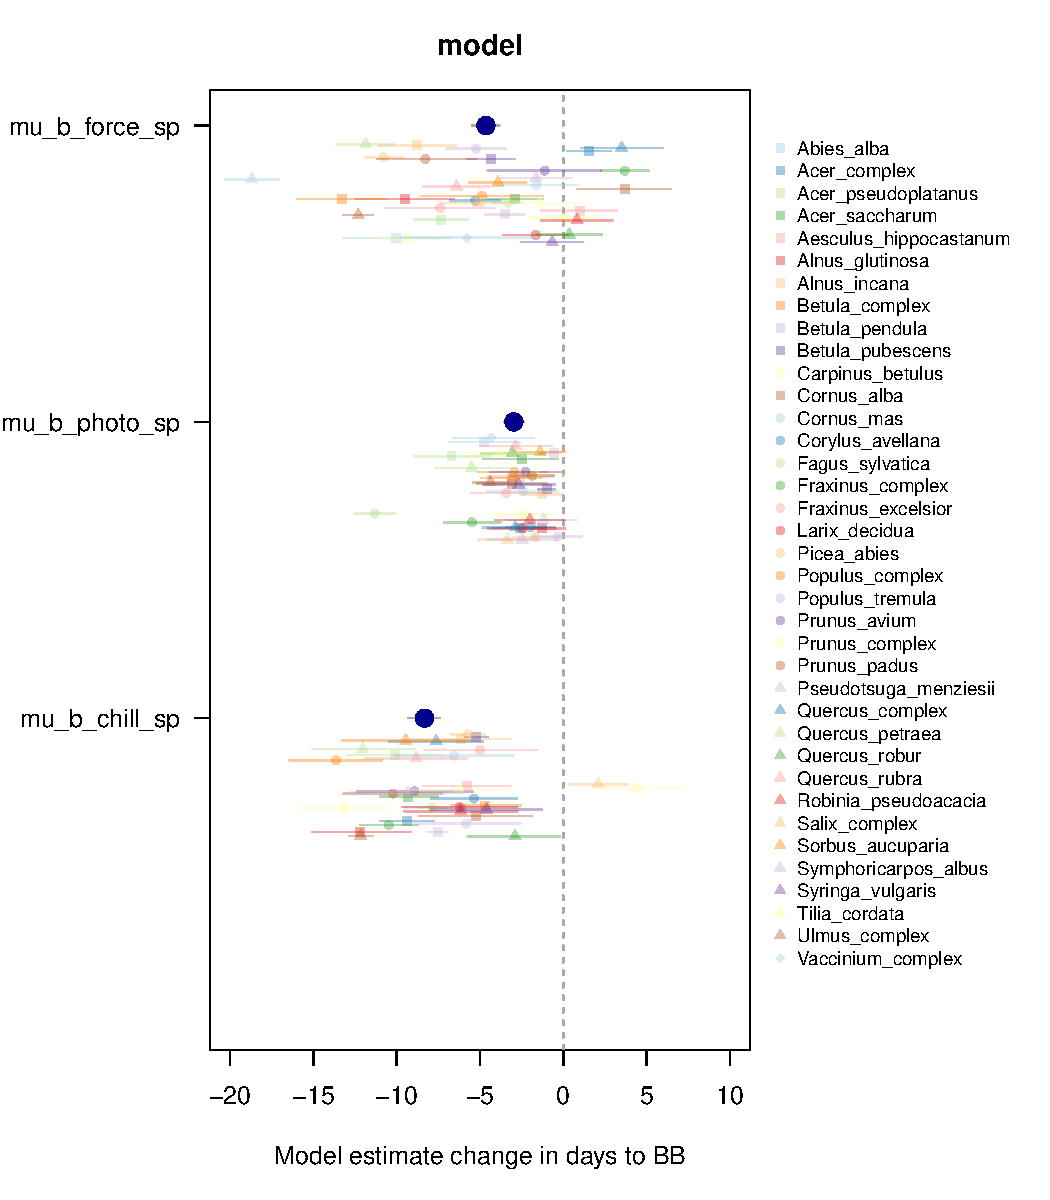
\includegraphics[width=0.75\textwidth]{..//..//analyses/bb_analysis/figures/muplotmodelspcom_expramp_fp_chillports.pdf}
\caption{Budburst model estimates}
\label{fig:mu}
\end{figure}


\begin{enumerate}
\item $\mu$ plots


\item  $\mu$ forecasting figures: spring x winter warming -- PEP climate range and experimental climate range
\item Species forecasting with PEP data: \emph{Betula, Fagus} ... need to think on which ones to use (x sites x species focus etc). ... Maybe show photoperiod one?
\item PEP data figure with environmental conditions: as in Cat's figure + OSPREE data + maybe foercasting (at 2C or such?)
\end{enumerate}


{\bf Supplemental figures/tables:}
\begin{enumerate}
\item Map of study locations, shading or symbol coding for number of cues (Lizzie)
\item Map of species forecasting to justify sites
\item Tables, yes.
\item Heat maps for the main data, including by actual study design and by calculated chilling (our calculations)
\item Photoperiod x latitude effects figure

\end{enumerate}
\end{enumerate}

\section{Reference list}

A few categories:\\

Papers about contrasting results over what cues matter from growth chamber studies: \cite{Basler:2012,Basler:2014aa,Caffarra:2011qf,Caffarra:2011a,Caffarra:2011b,Heide:2005aa,koerner2010b,Laube:2014a,vitasse2013,zohner2016}. Get Nanninga \emph{et al.} 2017: 'Increased exposure to chilling advances the time to budburst in North American tree species' and maybe Malyshev \emph{et al.} 2018 `Temporal photoperiod sensitivity and forcing requirements for budburst in temperate tree seedlings.'\\

Papers about declining sensitivities (Ailene will update this list): \cite{Rutishauser:2008fu,fu2015}. Also look for a Wang \emph{et al.} article `Impacts of global warming on phenology of spring leaf unfolding remain stable in the long run.' Vitasse paper on declining variation across elevation gradient. See \cite{yu2010}, but this is not temperate trees. \\

Papers about chilling units paper (Lizzie gets a list): Fu 2012 from OSPREE. \cite{harrington2015}\cite{lued2011,Luedeling:2011qe,Luedeling2013AgFM}\\

\bibliography{..//..//refs/ospreebibplus.bib}


\end{document}